\chapter{Latex} \label{ch:latex}
After learning about the content of a thesis, we will discuss how to present content using Latex. If you are familiar with Latex, you can skip this chapter; others will serve this as a time-saving starting point.


\section{Using this Template} \label{sec:Using_this_template}
This template is for your reference only. You do not have to adhere to this format and can change anything you like.

To use this template, configure some settings in the settings folder. Then, add your content in the content folder (you can use multiple \texttt{.tex} files, but it might be easier to only use one) and your references to \texttt{literature.bib} (see also Section \ref{sec:Citation}).

You can compile a pdf from \texttt{main.tex} either using \emph{pdflatex} or  \emph{latex + dvips + ps2pdf} (often configured as quick build). In an editor, e.g. Texmaker, you can set \texttt{main.tex} as master document, and thus compile from any file.


\section{Figures} \label{sec:Figures}
Figures are a very important tool to present content. A (good) visualization often helps the reader to understand your concepts. But do not forget to also explain in words what can be seen in the figure.

If you use \emph{pdflatex}, you can include \texttt{pdf} figures, and if you use \texttt{latex}, you can include \texttt{eps} figures (please always use vector graphics). To draw figures or edit plots you generate with MATLAB or Python, you can use Inkscape\footnote{\url{https://inkscape.org/en/}}.

Fig.~\ref{fig:scenario1} demonstrates how we include a figure. If you use \emph{latex + dvips + ps2pdf}, the \texttt{eps} is included and \emph{psfrag} replaces the letters \emph{a}, \emph{b}, and \emph{c} with latex code. If you use \emph{pdflatex}, you can save a \texttt{pdf} figure from Inkscape with the option to omit text in the pdf and create an additional \texttt{pdf\_tex} file, whose text will then be typeset with Latex (not shown here).

\begin{figure}[!htpb]
\centering
	\footnotesize
	\psfrag{a}[r][c]{Obstacle~1}	
	\psfrag{b}[l][c]{Obstacle~2}
	\psfrag{c}[c][c]{Obstacle~3}
	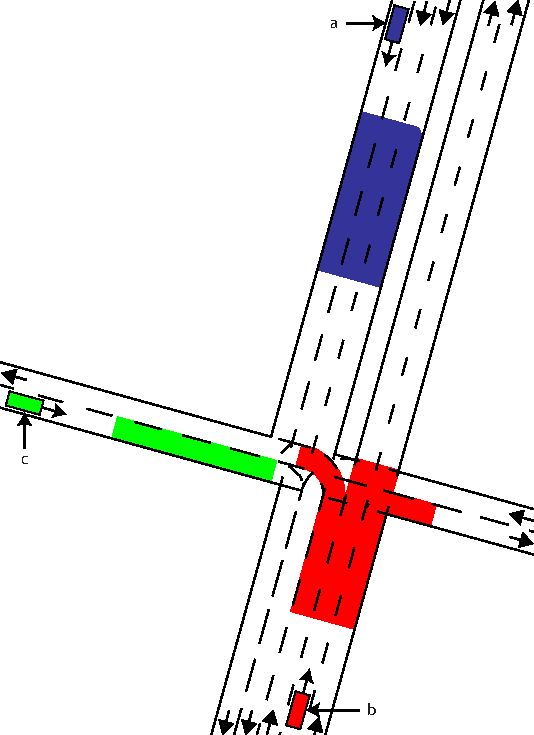
\includegraphics[width=0.4\columnwidth]{./figures/Scenario_Intersection_Occ_1,5-2,0s_final}
\caption{Occupancies of Obstacles~1, 2, and 3 in Scenario~I. The plot shows the initial configuration at $t_{0}$ and the predicted occupancies $\mathcal{O}(t)$ for ${t \in [t_{3}, t_{4}]}$.}
\label{fig:scenario1}
\end{figure}

\section{Math}
As an example, let us introduce $\mathcal{X}\subset\mathbb{R}^n$ as the set of feasible states $x$ and $\mathcal{U}\subset\mathbb{R}^m$ as the set of admissible control inputs $u$ of a system $f$, which is governed by the differential equation
\begin{equation}
	\begin{split}
	\dot{x}(t) &= f\big(x(t),u(t)\big). %\\
%	y&=g(x(t))
	\end{split}
	\label{eq:system}
\end{equation}

We assume that the initial time is $t_0 = 0$ and adhere to the notation $u([0, t_h])$ to describe a trajectory $u(t)\in\mathcal{U}$ for $t\in [0,t_h]$, $0<t_h$. Furthermore, $\chi\big(t_h,x(0),u([0,t_h])\big)\in\mathcal{X}$ denotes the solution of \eqref{eq:system} at time $t_h$ subject to $x(0)=x_0$ and $u([0,t_h])$.

Note that you should not reference an equation before introducing it. After giving the equation, you can refer to it, e.g., our system \eqref{eq:system} is awesome.


\section{Tables}
Tab.~\ref{tab:parameters} is an example of a nice table.

\begin{table}[!htb]\centering
\caption{Obstacle Parameters.}
\arstretch{1.3} 
\begin{tabular}{@{}llll@{}} \toprule
\textbf{Parameter} & \textbf{Variable} & \textbf{Parameter} &  \textbf{Variable} \\ \midrule
max. acceleration & $a_\mathrm{max}$ in $\unitfrac{m}{s^2}$ & Boolean for $C_\mathrm{back}$ & $b_\mathrm{back}$ \\ 
max. velocity & $v_\mathrm{max}$ in $\unitfrac{m}{s}$ & Boolean for $C_\mathrm{lane}$ & $b_\mathrm{lane}$ \\
switching velocity & $v_S$ in $\unitfrac{m}{s}$ & length & $l$ in $\unit{m}$ \\
speeding factor & $f_S$ & width & $w$ in $\unit{m}$ \\
\bottomrule
\end{tabular}
\label{tab:parameters}
\end{table}


\section{Algorithms}
Often, it will be helpful to describe your software by presenting pseudo code and explaining it (at least the significant lines). 

Alg.~\ref{alg:mainAlgorithm} shows the overall algorithm of \textit{SPOT}, which predicts the occupancy for a traffic participant up to the prediction horizon and can run in parallel for each traffic participant. First, the constraint management configures the parameters according to the set of last-measured states of the obstacle (line~\ref{alg:main_constraints}) as detailed in the next paragraph...

\begin{algorithm}
	\caption{Occupancy Prediction for an Obstacle}
	\begin{algorithmic}[1]
	\Require map
	\State parameters $\gets$ \Call{manageConstraints}{} \label{alg:main_constraints}
	\State reachableLanes $\gets$ \Call{reach}{map, parameters} \label{alg:main_reach}
	\ForAll{\Call{validAbstractions}{parameters}}
		\State $\mathcal{O}_{j}$ $\gets$ \Call{occupancy$_{j}$}{reachableLanes, parameters}\label{alg:main_abstractions}
	\EndFor
	\State \Return $\mathcal{O}$ $\gets$ \Call{intersect}{$\mathcal{O}_{j}$} \label{alg:main_intersect}
	\end{algorithmic}
	\label{alg:mainAlgorithm}
\end{algorithm}


\section{Citation} \label{sec:Citation}
For citations, we use a consecutively numbered citation style: bla \cite{latex} bla \cite{Koschi2017a, Althoff2017a} bla \cite{Paden2016}. To generate a bibliography file (the \texttt{.bib} file located in the folder content), you can use JabRef\footnote{\url{http://www.jabref.org/}}. Then, you run \textit{bibtex} and afterwards latex/pdflatex twice (as described in Sec.~\ref{sec:Using_this_template}).